\section{Polygon Representation}
\label{sec:polyrep}

\subsection{Basics}
\label{sec:polybasics}
In this section we state and prove several facts for $\eta$-near minimum cuts of a fractionally 2-edge-connected graph. All of the statements in this section are generalizable to the $(1+\eta)\alpha$ near minimum cuts of an $\alpha$-edge-connected graph (by rescaling) for $\eta \le 6/5$.  
\begin{definition}[Connected Component of Crossing Cuts]\label{def:conn-component-cuts}
	Given the set of $\eta$-near min cuts of a graph $G=(V,E)$, construct a graph where two cuts are connected by an edge if they cross. Partition this graph into maximal connected components. In the following, we will consider maximal connected components $\cC$ of crossing cuts and simply call them {\em connected components}.
	We say a connected component is a {\em singleton} if it has exactly one cut and a {\em non-singleton} otherwise. 
	
	For a connected component $\C$, let $\{a_i\}_{i \ge 0}$ be the coarsest partition of vertices $V$ such that for any $C\in \C$, either $a_i\subseteq C$ or $a_i\subseteq \overline{C}$. Each set $a_i$ is called an {\em atom} of $\C$ and we write  ${\cA}({\cal C})$ to denote the set of all atoms.
	
	Note for any atom $a_i \in \cA(\cC)$ which is an $\eta$-near min cut, $(a_i,\overline{a_i})$ is a singleton component, and is not crossed by any $\eta$-near min cut. Therefore $(a_i,\overline{a_i}) \not\in \cC$. 
	
	We can now represent any cut in $S \in \cC$ either by the set of vertices it contains or as a subset of $\cA(\cC)$. \textbf{In the following, we will often identify an atom with the set of vertices that it represents\footnote{For example, it will be convenient to write cuts as subsets of atoms. In this case the cut is the union of the vertices in those atoms.}.}
\end{definition}

 To study these systems, we will utilize the polygon representation of near minimum cuts defined in \cite{Ben97} and then extended in \cite{BG08}. Their work implies that any connected component $\mathcal{C}$ of crossing $\eta$-near minimum cuts has a polygon representation with the following properties, so long as $\eta \le \frac{2}{5}$: 

\begin{figure}
\begin{center}
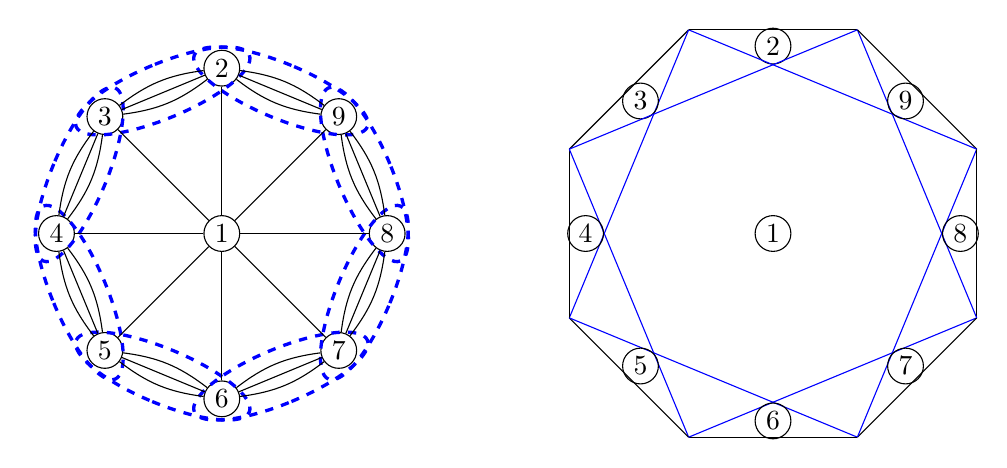
\begin{tikzpicture}[inner sep=1.7pt,scale=.7,pre/.style={<-,shorten <=2pt,>=stealth,thick}, post/.style={->,shorten >=1pt,>=stealth,thick}]
\tikzstyle{every node} = [draw, circle,color=black];
\begin{scope}[shift={(-5,0)}]
\foreach \i in {2,...,9}{
\path (\i*45:3) node  (a_\i) {\i};
}
\foreach \i in {0,...,7}{
\draw [color=blue,dashed,rotate around={22.5+45*\i:(22.5+\i*45:2.8)},line width=1.2] (22.5+\i*45:2.8) ellipse (.5 and 1.7);
}
%\draw [color=blue,dashed,rotate=45,line width=1.2] (45:2.8) ellipse (.7 and 1.7);
\path (0,0) node (c) {1};
\foreach \a/\b in {2/3, 3/4, 4/5, 5/6, 6/7, 7/8, 8/9, 9/2}{
\path (a_\a) edge  (a_\b) edge [bend left=15] (a_\b) edge [bend right=15] (a_\b) edge (c);
}
\end{scope}
\begin{scope}[shift={(5,0)}]
\foreach \i in {2,...,9}{
\draw (22.5+\i*45:4) -- (22.5+45+\i*45:4);
\path (\i*45:3.4) node  (a_\i) {\i};
\draw [color=blue] (22.5+\i*45:4) -- (22.5+90+\i*45:4);
}
\path (0,0) node (c) {1};
\end{scope}
\end{tikzpicture}
\end{center}
\caption[A Family of near Minimum Cuts with an Inside Atom]{%The left graph shows A 7-edge connected graph. The dashed blue lines show a cut class $\C$ of cuts of value at most 8, i.e., (1+1/7)-near minimum cuts. The right image shows the polygon representation of $\C$. The blue lines in the right image are the representing diagonals. This representation has 8 outside atoms and $\{1\}$ is the only inside atom. The system of near minimum cuts corresponding to sets $ (\{2,3\}, \overline{\{2,3\}}), \ldots, (\{8,9\},\overline{\{8,9\}}), (\{9,2\}, \overline{\{9,2\}})$ shows an $8$-cycle for the inside atom $\{1\}$.
Consider the graph on the left and suppose that every edge $e$ has fractional value $x_e =1/7$. This graph then has min cut value 2, with cuts of fractional value at most $2 + 1/7$ circled in blue. Note that this is a connected family $\C$ of near-min cuts, since every adjacent pair of blue cuts cross each other. The right image shows the polygon representation of $\C$. The blue lines in the right image are the representing diagonals. This representation has 8 outside atoms and $\{1\}$ is the only inside atom. The system of near minimum cuts corresponding to sets $ (\{2,3\}, \overline{\{2,3\}}), \ldots, (\{8,9\},\overline{\{8,9\}}), (\{9,2\}, \overline{\{9,2\}})$ shows an $8$-cycle for the inside atom $\{1\}$. See \autoref{def:kcycle}.}
\label{fig:polygonrepresentation}
\end{figure}

\begin{enumerate}
	\item A polygon representation is a convex regular polygon with a collection of \textit{representing diagonals}. All polygon edges and diagonals are drawn using straight lines in the plane. The diagonals partition the polygon into \textit{cells}. 
	\item Each atom of $\C$ is mapped to a cell of the polygon.  If one of these cells is bounded by some portion of the polygon boundary it is {\em non-empty} and we call its atom an \textit{outside atom}. We call the atoms of all other non-empty cells \textit{inside atoms}. Note that some cells may not contain any atom. WLOG label the outside atoms $a_0,\dots,a_{m-1}$ in counterclockwise order, and label the inside atoms arbitrarily. We also label points of the polygon $p_0,\dots,p_{m-1}$ such that outside atom $a_i$ is on the side $(p_i,p_{i+1})$ and $a_0$ is on the side $(p_{m-1},p_0)$. (In future sections we will refer to the special atom called the root, and if it is an outside atom WLOG we will label $a_0$ as the root.)
	\item No cell has more than one incident outer polygon edge.
	\item Each representing diagonal defines a cut such that each side of the cut is given by the union of the atoms on each side. Furthermore, the collection of cuts given by these diagonals is exactly $\mathcal{C}$. 
\end{enumerate}


%We will deal solely with connected components of cuts. In each connected component, we will effectively delete some cuts and then merge others into laminar families. 
The following fact follows immediately from the above discussion:
\begin{fact}
\label{fact:atLeast2Outside}
Any cut $S\in \cC$ (represented by a diagonal of $P$) must have at least two outside atoms.
\end{fact}


\begin{definition}[Outside atoms]
	For a polygon $P$ and a set $S$ of atoms of $P$, we write $O_P(S)$ to denote the set of outside atoms of $P$ in $S$; we drop the subscript when $P$ is clear from context. We also write $O(P)$ (or $O(\cA(\cC))$ where $\cC$ is the connected component of $P$) to denote the set of all outside atoms of $P$.
	
	Note that, given $S \in \cC$, since $S$ may be identified with a set of atoms, $O(S)$ is also well defined. 
\end{definition}



The following observation follows from  the fact that cuts correspond to straight diagonals in the plane and the polygon $P$ is regular:
%\Shayan{We need to justify this observation. Are we using it?}
\begin{observation}[{\cite[Prop 19]{BG08}}] \label{obs:Ocross}
	If $S,S'\in {\cal C}$ cross then $O(S)$ and $O(S')$ cross, and $O(S \cup S') \not= O(P)$.
\end{observation}


\cref{lem:mincutBshowsup} is used in the proof of \cref{lem:extendedprop20}, and depends on the following:

%The following is proved in \cite[Lem 4.1.7]{Ben97}
\begin{theorem}[{\cite[Lem 4.1.7]{Ben97}}]\label{thm:BenCC'}
	Let $\C,\C'$ be two (distinct) connected components of crossing cuts for a family of cuts of $G=(V,E)$. Then, there exists an atom $a\in \cA(\C)$ and $a'\in \cA(\C')$ such that $a\cup a'=V$. 
\end{theorem}


\begin{lemma}\label{lem:mincutBshowsup}
Consider the set of $\eta$-near minimum cuts (NMCs) of $G$ and let $\C$ be a connected component. Let $B\subset\cA(\C)$ be an $\eta$-NMC such that $1<|B|<|\cA(\C)|-1$. Then, $B\in \C$. 
\end{lemma}
\begin{proof}
For the sake of contradiction, suppose $B\notin \C$. Since $B$ is an $\eta$-NMC, it is in some connected component of cuts, say $B\in \C'$, where $\C\ne \C'$. Then, by \cref{thm:BenCC'} there exist atoms $a\in\cA(\C),a'\in\cA(\C')$ such that $a\cup a'=V$.
Observe that by the definition of atoms, each of $a,a'$ is contained in either $B$ or $\overline{B}$. Without loss of generality assume $a\subseteq B$ and $a'\subseteq \overline{B}$. But then, $a\neq B$ since $|B|>1$. So, $a\cup a'\neq V$ which is a contradiction. 
\end{proof}






%\subsubsection{Modified cactus representation}
%
%First we recall the definition of a cactus graph:
%
%\begin{definition}[Cactus Graph]
%\label{def:cactus}
%A {\em cactus graph} is a graph with no cut edges {and} in which no two simple cycles share an edge. \end{definition}
%
%In \cite{Ben97}, it is shown that any collection of cuts admits a modified cactus representation. In particular:
%
%\begin{theorem}[{\cite{Ben97}}]
%\label{thm:tree-representation}
%Let $\cF$  be a collection of cuts of $G=(V,E)$. %, and let $P_i$ be the partition of $V$ corresponding to $\cA(\C)$.
%There exists a cactus $K=(N,E')$ and a mapping $\phi: N \to 2^V$ such that: 
%\begin{enumerate}
%\item $K$ has no cycle of length 3.
%\item There is a 1-to-1 correspondence between the connected components $\cC$ of $\cF$ and the cycles of $K$. In particular, if a connected component $\cC$ and a cycle $L$ are in correspondence, then if $\cC$ has atoms $a_1,\dots,a_k \subseteq 2^V$ (i.e. this forms the coarsest partition of the vertices in $\cC$ as in \cref{def:conn-component-cuts}), $L$ has $k$ vertices and we can order them $v_1,\dots,v_k$ such that $\phi(v_i) = a_i$.
%\item All pairs of atoms $A\in \cA(\C)$ and $B\in \cA(\C')$ with $\C\neq \C'$ that are mapped to a coinciding vertex of the cactus satisfy $\phi(A) \cup \phi(B) = V$.
%\end{enumerate}
%\end{theorem}



%While \cref{sec:poly} does not depend upon any particular random spanning tree distribution, \cref{thm:main} relies heavily on the use of $\lambda$-uniform spanning tree distributions proved in ~\cite{KKO21}.
%For a vector $\lambda:E\to\R_{\geq 0}$, a $\lambda$-uniform distribution $\mu_\lambda$ over spanning trees of $G=(V,E)$ is a distribution where for every spanning tree $T\subseteq E$, $\PP{\mu}{T}=\frac{\prod_{e\in T} \lambda_e}{\sum_{T'} \prod_{e\in T'} \lambda_e}$.
%Now, find a vector $\lambda$ such that for every edge $e\in E$, $\PP{\mu_\lambda}{e\in T}=x_e(1\pm\eps)$, for some $\eps<2^{-n}$. Such a vector $\lambda$ can be found using the multiplicative weight update algorithm \cite{AGMOS10} or by applying interior point methods \cite{SV12} or the ellipsoid method \cite{AGMOS10}. (We note that the multiplicative weight update method can only guarantee $\eps<1/\text{poly}(n)$ in polynomial time.)
%\begin{theorem}[\cite{AGMOS10}]
%\label{thm:maxentropycomp}
%Let $z$ be a point in the spanning tree polytope (see \eqref{eq:spanningtreelp}) of a graph $ G=(V, E)$.
%For any $\eps>0$, a vector $\lambda:E\to\R_{\geq 0}$ can be found such that the corresponding $\lambda$-uniform spanning tree distribution, $\mu_\lambda$, satisfies
%%we define the exponential family distribution
%%$$\tilde{p}(T):=\frac{1}{P}\exp(\sum_{e\in T} \tilde{\gamma}_e)$$ for
%%all $T\in {\cal T}$ where $$P:=\sum_{T\in {\cal T}}\exp(\sum_{e\in T}
%%\tilde{\gamma}_e)$$ then, for every edge $e\in E$,
%$$%\tilde{z}_e :=
%\sum_{T\in {\cal T}: T \ni e} \PP{\mu_\lambda}{T}  \leq (1+\varepsilon)z_e,\hspace{3ex}\forall e\in E,$$
%i.e., the marginals are approximately preserved.  In the above ${\cal T}$ is the set of all spanning trees of $(V,E)$. The running
%time is polynomial in $n=|V|$, $- \log \min_{e\in E} z_e$ and $\log(1/\eps)$.
%\end{theorem}





\subsection{Our polygon notation and the root}\label{sec:polynotation}

All statements in the previous section do not depend on which side of each diagonal we consider. The ambiguity on the sides of the cut considered makes it difficult to define a consistent orientation on the polygon, for example to say whether a cut $A,\overline{A}$ crosses $B,\overline{B}$ ``on the left" or ``on the right." Motivated by this, we identify every cut with the side that does not contain $u_0,v_0$. This has the added benefit of allowing us to apply \cref{lem:treeconditioning} to every cut considered. For every polygon $P$, we call the unique atom $r$ containing $u_0,v_0$ \textit{the root}.  

Recall that, for $\eta>0$, we write $\cN_\eta  \subseteq 2^{V \smallsetminus \{u_0,v_0\}}$ to denote the family of all $\eta$-NMCs of $G_{/e_0}$. %We will always identify each cut  $\delta(S)$ with the side $S$ that does not contain $\{u_0,v_0\}$. 
If $\eta$ is clear in context, we drop the subscript of $\cN_\eta$.
Throughout the paper, we will need to show that various sets $A,B \subseteq V\smallsetminus \{u_0,v_0\}$ cross. Since $u_0, v_0 \in \overline{A \cup B}$ to verify that a pair of sets $A$ and $B$ cross, it suffices to check the three conditions in the following fact.
%By \cref{fact:nou0v0cross} in such cases we only need to verify that $A\cap B,A\smallsetminus B, B\smallsetminus A$ are non-empty (since $A,B$ do not contain $u_0,v_0$). 
\begin{fact}\label{fact:nou0v0cross}
For $A,B\subseteq V\smallsetminus\{u_0,v_0\}$, $A,B$ cross iff
$$A\cap B, A\smallsetminus B, B\smallsetminus A\neq\emptyset.$$	
\end{fact}

As above, unless otherwise specified, we let $\cC$ be a connected component  of cuts in $\cN_\eta$ with corresponding  polygon $P$ for $\eta \leq 1/10$. Again, call the {\em outside} atoms (of $P$) $a_0,\dots,a_{m-1}$, ordered counter-clockwise though these are not necessarily all the atoms in $P$. Note that the root $r$ is not necessarily an outside atom, but if it is, it is the atom labelled $a_0$. 

We use the existence of the root to prove the following two facts. The first fact is a consequence of \cref{obs:Ocross}:

\begin{fact}\label{fact:union-not-everything}
Let $S,S' \in \cC$. Then, $O(S \cup S') \not= O(\cA(\cC))$. 
\end{fact}
\begin{proof}[Proof sketch]
If $S,S'$ are (the non-root) sides of two diagonals of a polygon and there is an atom $r$ which is in neither of them, then there must be a polygon point which is in neither of them. 
%To see this formally, not that if $S,S'$ cross then by \cref{obs:Ocross} we are done. Therefore, we may assume that $A \cap B = \emptyset$, $A \subseteq B$, or $B \subseteq A$. The latter two cases are immediate. So, assume $A \cap B = \emptyset$. 
\end{proof}

The following lemma is the main reason why we can treat each polygon separately in constructing the slack vector mentioned in \cref{sec:overview}. In \cref{sec:twoside}, we are careful to only define positive slack on edges of a polygon that do not have an endpoint in its root.

\begin{fact}\label{fact:edges-internal-to-one-poly}
For any edge $e=\{u,v\}$, there is at most one polygon in which the endpoints of $e$ lie in two different atoms which are not the root of their respective polygons.
\end{fact}
\begin{proof}
	Suppose not, and let $P,P'$ be two polygons in which $u$ and $v$ lie in different atoms that do not contain $r$. By \cref{thm:BenCC'}, there exists an atom $a \in P,a' \in P'$ such that $a \cup a' = V$. Since $u,v$ lie in different atoms (and the atoms of a polygon partition $V$) in both $P,P'$ it must be that (WLOG) $u \in a, v \in a'$. However, since $a \cup a' = V$, $u_0,v_0$ lies in $a$ or $a'$, so either $a$ is the root of $P$ or $a'$ is the root of $P'$, which is a contradiction. 
\end{proof}

%We will call $r$ the root. % such that $a_0$ is the unique atom that contains $e_0=\{u_0,v_0\}$. %We identify each cut in ${\cal C}$ with the side of its representing diagonal that does not contain the root.



We will use {\em``left" synonymously with ``clockwise"} and {\em``right" synonymously with ``counter-clockwise."} 


\begin{definition}[Near min cut notation]
	We will interchangeably refer to a set $S\in\cN_\eta $  by specifying the extreme outside atoms it contains or by specifying the polygon points defining its diagonal. For the former, if $S=(a_l,a_r)$, then  $a_l$ is the leftmost outside atom in $S$ and $a_r$ is the rightmost outside atom in $S$. For the latter, if $S=(p_l,p_r)$, then $p_l$ is the polygon point immediately to the left of $a_l$ and $p_r$ is the polygon point immediately to the right of $a_r$. 
\end{definition}




%For every pair of polygon points $p,q$, consider the two regions defined by the diagonal connecting $p$ to $q$. Let $S=(p,q)$ denote the set of atoms in the region not containing the root. By convention we will write $S=(p_l,p_r)$ such that moving counterclockwise from $p_l$ to $p_r$ we hit all the outside atoms of $S$. For convenience we will also sometimes refer to $S$ as $S=(a_l,a_r)$ where $a_l,a_r$ are outside atoms and $a_l$ is to the left of $a_r$ analogously to above.

%We say an outside atom $a_i$ is \textit{to the left} of another outside atom $a_j$ if $i < j$ and \textit{to the right} otherwise. 

\begin{definition}[$L(p)$, $R(p)$]
For a polygon point $p_i$, let $L(p_i)$  be the largest cut in $\cN_\eta$ containing $a_{i}$ and not $a_{i+1}$ which is crossed on both sides. Let $R(p_i)$ be the largest cut in $\cN_\eta$ containing $a_{i+1}$ and not $a_{i}$ which is crossed on both sides. (Note that $L(p_i),R(p_i)$ do not necessarily exist). See \autoref	{fig:LpRp}.
\end{definition}


 %For example, see \cref{fig:opt-augmentation}. 

%\begin{figure}[htb]
%\begin{center}
%\begin{tikzpicture}[inner sep=1.7pt,scale=.7,pre/.style={<-,shorten <=2pt,>=stealth,thick}, post/.style={->,shorten >=1pt,>=stealth,thick}]
%
%\node at (-3,-2.5) () {$S_L$};
%\node at (3.5,1.5) () {$S_R$};
%
%\node at (1,-3.5) () {$S$};
%
%\tikzstyle{every node} = [draw, circle,color=red];
%\foreach \i in {1,...,8}{
%\path (22.5+\i*45:3) node  (a_\i) {};
%}
%
%\path (a_5) edge [thick, bend right=25, green] (a_4);
%\path (a_5) edge [thick, bend right=15, green] (a_3);
%
%\path (a_7) edge [thick, bend left=25, blue] (a_8);
%\path (a_7) edge [thick, bend left=15, blue] (a_1);
%
%\path (a_7) edge [thick, bend right=15, red] (a_4);
%\path (a_6) edge [thick, bend left=15, red] (a_1);
%\path (a_5) edge [thick, bend right=15, red] (a_2);
%
%\draw [color=black,rotate around={45*4.5:(4.3*45:1.6)},line width=1.2] (4*45:0.8) ellipse (0.9 and 2.7);
%\draw [color=black,rotate around={45*8.5:(1*45:1.6)},line width=1.2] (4.25*45:-2.1) ellipse (0.9 and 2.7);
%
%\draw [color=black,rotate around={45*6.5:(4.3*45:1.6)},line width=1.2] (1.1*45:1.5) ellipse (0.9 and 2.7);
%
%\foreach \a/\b in {1/2, 2/3, 3/4, 4/5, 5/6, 6/7, 7/8, 8/1}{
%\path (a_\a) edge  (a_\b);
%}
%
%\end{tikzpicture}
%\end{center}
%%\caption{$S$ is crossed on the left by $S_L$ and on the right by $S_R$. In green are edges in $\delta(S)^\leftarrow$, in blue edges in $\delta(S)^\rightarrow$, and in red are edges in $\delta(S)^\circ$. }
%\label{fig:crossed-both-sides}
%\end{figure}

The following definitions make formal the notion of ``crossed on one side" and ``crossed on both sides" (introduced in \cref{sec:overview}) for polygons with inside atoms.

\begin{definition}[Left, Right Crossing]
Let $S,S'\in \cC$ such that $S'$ crosses $S$.
For such a pair, we say \textit{$S'$ crosses $S$ on the left} if the leftmost (clockwise-most) outside atom of $O(S' \cup S)$ is in $S'$. %(see \cref{fact:contiguous}).
 Otherwise, we say that \textit{$S'$ crosses $S$ on the right}. Note that by \cref{obs:Ocross}, $O(S),O(S')$ cross. 
%See \cref{fig:polygonexample} for an example.
\end{definition}
\begin{definition}[Crossed on one, both sides]
\label{defn:crossedonetwo}
We say a cut $S$ is \textit{crossed on both sides} if it is crossed by a cut (in $\cC$) on the left and a cut (in $\cC$) on the right and we say $S$ is {\em crossed on one side} if it is crossed only on the left or only on the right. 
\end{definition}

\begin{definition}[$\cN_{\eta,\le 1},\cN_{\eta,1},\cN_{\eta,2}$]
	Let $\cN_{\eta,2} \subseteq \cN_\eta$ be the set of cuts which are crossed on both sides in their respective polygons. Let $\cN_{\eta,1} \subseteq \cN_\eta$ be the set of cuts that are crossed on one side in their respective polygons and finally let $\cN_{\eta,\le 1} = \cN_\eta \smallsetminus \cN_{\eta,2}$ (i.e. the set of cuts which are crossed on one side or not crossed at all).
\end{definition}


Here we give an alternate set-theoretic characterization of $\cN_{\eta,2}$.

\begin{lemma}\label{lem:characterize-N2}
Let $C \in \cN_\eta$. Then, $C \in \cN_{\eta,2}$ if and only if there exist two cuts $A,B \in \cN_\eta$ which cross $C$ such that $(A \smallsetminus C) \cap (B \smallsetminus C) = \emptyset$. 	
\end{lemma}
\begin{proof}
The only if follows from \cref{lem:nointersectionLR}. So, assume there exist two cuts $A,B \in \cN_\eta$ which cross $C$ such that $(A \smallsetminus C) \cap (B \smallsetminus C) = \emptyset$. We will show $C \in \cN_{\eta,2}$. 

Since $A$ and $B$ both cross $C$, it must be that $C,A,B$ are in the same connected component of cuts $\cC \subseteq \cN_\eta$ (i.e. including all cuts in $\cN_{\eta,2}$). Let $P$ be the corresponding polygon.
	
	%By \cref{obs:Ocross}, $O(A)$ and $O(C)$ cross and $O(B)$ and $O(C)$ cross. \anna{Why do you need the last sentence?} 
	Suppose by way of contradiction that $A,B$ both crossed $C$ on the left (if they both cross on the right the argument is similar). Then $A,B$ must both contain the outside atom immediately to the left of the leftmost atom of $C$, which contradicts $(A \smallsetminus C) \cap (B \smallsetminus C) = \emptyset$.
\end{proof}

Consequently, we can give an alternate characterization of $\cN_{\eta,1}$ as the sets which are crossed but are not in $\cN_{\eta,2}$. This will be relevant in \cref{app:oneside}. 

\begin{definition}[$\cC_{2}$]
	For a connected component of cuts $\cC \subseteq \cN_\eta$, let $\cC_{2} = \cC \cap \cN_2$. 
\end{definition}


The following definition is quite important throughout our paper as it is used to specify the set of bad events we use to construct our slack vector (see \cref{sec:overview} for a gentle introduction):

 \begin{definition}[$S_L$, $S_R$]\label{def:SLR}
 For $S \in \cC_2$ let $S_L$ be the near minimum cut crossing $S$ on the left which minimizes $|O(S \cap S_L)|$. If there are multiple sets crossing $S$ on the left with the same minimum intersection, choose the smallest one to be $S_L$. Similarly, let $S_R$ be the near min cut crossing $S$ on the right which minimizes $|O(S \cap S_R)|$, and again choose the smallest set to break ties. See \autoref{fig:S-SR-SL}.
 
 %Equivalently, given $S=(p_l,p_r)$, let $r'$ be the first index in the counterclockwise order starting from $l$ such that there exists a cut $S'$ with rightmost polygon point $p_{r'}$ which crosses $S$ on the left. In such a case, let $S_L$ be the cut minimizing $|O(S_L)|$ among all cuts with rightmost polygon point $p_{r'}$ that cross $S$ on the left. We can define $S_R$ similarly.

% For any set $S$ crossed on both sides such that $S_L, S_R$ cross $S$ on the left and right respectively and minimize their intersections with $S$, 


 \end{definition}
 






%\begin{figure}
%\begin{center}
%\begin{tikzpicture}[inner sep=1.7pt,scale=1,pre/.style={<-,shorten <=2pt,>=stealth,thick}, post/.style={->,shorten >=1pt,>=stealth,thick}]
%\tikzstyle{every node} = [draw,circle,color=black];
%\foreach \i in {0,...,7}{
%\draw (22.5+\i*45:4) -- (22.5+45+\i*45:4);
%\path (90+\i*45:3.4) node  (a_\i) {$a_\i$};
%\draw [color=blue] (22.5+\i*45:4) -- (22.5+90+\i*45:4);
%}
%\path (0,0) node (c) {1};
%\path (90:3.4) node[fill=lightgray]  (a_0) {$a_0$};
%\end{tikzpicture}
%\end{center}
%\caption{In this example, $a_0...a_7$ are the outside atoms, and recall that we identify every diagonal with the side not containing the root. Suppose that $a_0$ is the root (note that the root is not necessarily an outside atom). Then, in this example, $\{a_1,a_2\}$ and $\{a_1...a_6\}$ and are only crossed on the right. $\{a_6,a_7\}$ and $\{a_2...a_7\}$ are only crossed on the left. All other cuts are crossed on both sides. Here we say $a_4$ is to the left of $a_5$ and $a_6$ is to the right of $a_5$. $a_0$ is not comparable to any other atom.}
%\label{fig:polygonexample}
%\end{figure}





\subsection{Properties of inside atoms}

Before proving some new properties of the polygon representation we recall some basic properties of inside atoms from \cite{BG08}:

\begin{definition}[{\cite[Definition 3]{BG08}}]\label{def:kcycle}
A family of sets $C_1,\dots,C_k\subseteq V$, for some $k \ge 3$, forms a $k$-cycle if
\begin{itemize}
\item $C_i$ crosses both $C_{i-1}$ and $C_{i+1}$ (we treat $C_{k+1}$ as $C_1$ and $C_{0}$ as $C_k$);
\item $C_i\cap C_j=\emptyset$ for $j\neq i-1, i$ or $i+1$; and
\item $\bigcup_{1\leq i\leq k} C_i \neq V$.
\item If $k=3$, we have the additional condition $(C_i \cap C_{i+1}) \not\subseteq C_{i-1}$ for $i \in \{1,2,3\}$.
\end{itemize}
\end{definition}


\begin{lemma}[{\cite[Lemma 22]{BG08}}]\label{lem:no-kcycle}
%If  $\eta > \frac{2}{k}$.	
Any $k$-cycle formed by cuts in a connected component ${\cal C}$ of $\eta$-near min cuts satisfies $k\geq 2/\eta$. (Note if $\eta = 0$ then no $k$-cycle exists.)
\end{lemma}

Therefore, for all $2/5$-near min cuts, there are no cycles with length less than 5.
%Generally speaking, since we assume $\eta\ll 1$, the above lemma implies that any $k$-cycle of ${\cal C}$ satisfies $k\gg 3$. 
%This definition gives rise to the formal definition of inside atoms and a related fact:
\begin{lemma}[{\cite[Def 4]{BG08}}]\label{def:inside}
	An atom $a\in \cA(\cC)$ is an inside atom (in the representation defined above) if and only if there is a $k$-cycle $C_1,\dots,C_k\in {\cal C}$, such that $a \cap C_i=\emptyset$ for all $1 \le i \le k$. 
\end{lemma}
See \autoref{fig:polygonrepresentation} for an example of an inside atom and a cycle.

\begin{fact}\label{lem:adjoutsidekcycle}
Let $C_1,\dots,C_k$ be a $k$-cycle for a connected component $\C$ with polygon representation $P$ and $k \ge 5$. For any adjacent pair of outside atoms $a,b\in O(\cA(\cC))$, there is a $1\leq j\le k$ such that $a,b\in C_j$.	
\end{fact}
\begin{proof}
Since $a$ is an outside atom, there is a cut $C_i$ for some $1\leq i\leq k$ such that $a\in C_i$ (otherwise $a$ would be an inside atom). If $b\in C_i$ we are done. Otherwise, $a$ is a rightmost or leftmost outside atom in $C_i$. But then, since $C_i$ is crossed by $C_{i-1}$ and $C_{i+1}$ and $C_{i-1} \cap C_{i+1} = \emptyset$, it follows from \cref{obs:Ocross} (and the fact that both $C_{i-1},C_{i+1}$ contain at least two outside atoms) that either $a,b \in C_{i-1}$ or $a,b \in C_{i+1}$.
%Label the outside atoms of $P$, $o_0,\dots,o_{n-1}$ in clockwise order. WLOG let $C_1,\dots,C_k$ be ordered clockwise such that $O(C_i) = [o_{\ell_i},o_{r_i}]$ such that $\ell_i < r_i$, and $\ell_i < \ell_{i+1} < r_i < r_{i+1} \forall i$ (all mod $n$). 
%WLOG $b$ is the outside atom immediately counterclockwise of $a$. Since $a$ is an outside atom, there is a cut $C_i$ for some $1\leq i\leq k$ such that $a\in C_i$ (otherwise $a$ would be an inside atom). If $b\in C_i$ we are done. 
%Otherwise, $C_i$ is crossed by $C_{i-1}$ and $C_{i+1}$, and say the former crosses $C_i$ such that in the interval $O(C_{i-1} \cup C_i)$, $C_{i-1}$ contains the outside atom furthest counterclockwise. Since $C_{i-1},C_i$ cross, by \cref{obs:Ocross} their outside atoms cross, so $C_{i-1}$ must have both $a,b$.
\end{proof}

\subsection{New properties of polygon representations}
\label{sec:polygonsnewproperties}

The following lemmas build on \cite{Ben95,BG08}. 
\cref{prop20} is a key property of polygons which \cref{lem:extendedprop20} extends: %Some of the statements may have implicitly appeared in those works.


%\begin{lemma}\label{thm:halfplanes}
%Let $ \eta \le  2/5$ and let $P$ be the polygon representation for a connected component $|{\cal C}|$ of at least two $\eta$-NMCs of a (fractionally) 2-edge-connected graph. 
%
%Let $\cH$ be a set of half-planes where each half-plane is one side of a diagonal $D$ of $P$ (corresponding to a represented near min cut) extended to infinity. Suppose that the polytope $\bigcap_{H \in \cH} H$ is non-empty and is entirely contained in the closed set $P$. Let $v_0,\dots,v_{\ell-1}$ be the vertices of $P$ arranged cyclically counterclockwise. Then, perhaps after renaming, it is defined by $\ell$ half-planes $H_0,\dots,H_{\ell-1} \in \cH$ with corresponding diagonals $D_0,\dots,D_{\ell-1}$, where $v_i$ is at the intersection of $D_i$ and $D_{i+1 \pmod{\ell}}$. Note that a segment of each of these diagonals forms a unique edge of the polytope.
%
%%Suppose $H$ is a bounded non-empty intersection of half-planes which lies inside $P$.
% %where each half-plane corresponds to one side of a diagonal $D$ of $P$. If $H$ has $\ell$ vertices, then WLOG it is defined by 
%%If $H$ does not contain any side of $P$ (equivalently, it does not any contain any outside atom) and 
%If $\ell<1/\eta$ then $H$ does not contain any atoms.
%%	The boundary of any non-empty inside cell of the polygon $P$ corresponding to a connected component $\C$ of $\eta$-NMCs   is defined by at least $\Omega(1/\eta)$ diagonals.
%\end{lemma}
%\begin{proof}
%%Define $C_0,\dots,C_{\ell-1} \subseteq V$ such that $C_i$ is all atoms which are not in the halfplane $H_i$. Without loss of generality assume there are no two sets $C_i,C_j$ such that $C_i \subseteq C_j$\footnote{This is because if $C_i \subseteq C_j$ then $H_j \cap P \subseteq H_i \cap P$ which means $H_i$ is redundant in defining $H$.}. 
%%
%%First observe that $H$ is a 2-dimensional polytope and therefore without loss of generality we can assume the diagonals $D_0,\dots,D_{\ell -1}$ are ordered such that the vertices of the polytope $v_0,\dots,v_{\ell-1}$ are arranged cyclically counterclockwise where $v_i$ is the intersection of $D_i$ and $D_{i+1}$ 
%For the rest of the proof take all indices mod $\ell$. We will call a vertex $v_i$ \textit{external} if $D_{i}$ and $D_{i+1}$ intersect at a vertex of $P$ and \textit{internal} otherwise.
%
%We prove the claim by induction over $r$ that if $H$ has $r$ external vertices and $\ell+r < 2/\eta$, then $H$ contains no atoms. This will suffice to prove the theorem because assuming $\ell < 1/\eta$, we have $\ell+r<2/\eta$ (using that $r\leq \ell$).
%
%First assume $r=0$. Then, $C_{i}$ crosses $C_{i+1}$ for all $i$. By way of contradiction suppose $H$ contains an (inside) atom $a$. We claim that for every $i,j$ where $j \not\in \{i-1,i,i+1\}$, we have $C_i \cap C_j = \emptyset$. Suppose not. Then since $C_i \not\subseteq C_j$,  $C_j \not\subseteq C_i$, $a \not\in C_i,C_j$, it follows that $C_i,C_j$ cross and therefore the diagonals $D_i,D_j$ intersect in the interior of $P$, which is a contradiction.%. Now $D_0,\dots,D_i,D_j,\dots,D_{\ell-1}$ contains $H$ and has no external vertices and thus contradicts the minimality of $H_0,\dots,H_{\ell-1}$.  
%
%Therefore by minimality, $C_i \cap C_j = \emptyset$ if $j \not= i-1,i$ or $i+1$. So, $C_0,\dots,C_{\ell-1}$ is a $k$-cycle for $a$: since there are no external vertices, $C_i$ crosses $C_{i+1}$ for all $i$, and $\bigcup_{i=0}^{\ell-1} C_i \not= V$ since $a \not\in C_i$ for all $i$. But by \cref{lem:no-kcycle}, $\ell \ge 2/\eta$, which is a contradiction.
%
%Now, suppose the claim is true when the number of external vertices is at most $r$; we will prove it holds when the number is $r+1$.  
%
%Again, by way of contradiction suppose there is an inside atom $a$ in $H$. Then there is a $k$-cycle for $a$ in $\cC$,  say $L_1,\dots,L_k$. Now pick an arbitrary external vertex $v_i$ of $H$. Let $o_l,o_r \in O(\cA(\cC))$ be the adjacent outside atoms immediately clockwise and counterclockwise of $v_i$. Therefore, since $k \ge 4$, by \cref{lem:adjoutsidekcycle}, there exists some $j$ such that $o_l,o_r \in L_j$. Let $H_{\ell}$ be the halfspace corresponding to the side of $L_j$ containing $a$. Now consider the set of halfspaces $H_0,\dots,H_{\ell-1},H_{\ell}$. Note that $H'=\bigcap_{i=0}^{\ell} H_i \subsetneq H$ because $v_i \not\in H_\ell$. Therefore, $H'$ has at least one fewer external vertex and no sides of the polygon. Since $\ell+1+(r-1) \le 2/\eta$, by the induction hypothesis, $H'$ has no inside atoms which is a contradiction with the existence of $a$. 
%\end{proof}

%\begin{lemma}[{\cite[Lemma 12]{BG08}}]\label{lem:kcycle}
%	Let $S \in {\cal C}$ and $f \in S$ be an inside atom. Let $C_1...C_k$ be a cycle for $f$. Then there exists an $i$ such that $C_i \subset S$. 
%\end{lemma}


\begin{proposition}[{\cite[Proposition 20]{BG08}}]\label{prop20}
For any connected component ${\cal C}$ of $\eta$-near min cuts with $\eta \leq 2/5$ with polygon representation $P$, and any $S_1, S_2 \in \mathcal{C}$ with $S_1 \not= S_2$ we have $O_P(S_1) \neq O_P(S_2)$.
\end{proposition}
%\anna{The polygon representation is unique, right? Also, are atoms $\eta$ near mincuts?}

\begin{lemma}\label{lem:extendedprop20}
Let $P$ be the polygon representation  for a connected component $|{\cal C}|>1$ of $\eta$-NMCs of a (fractionally) 2-edge connected graph $G$ with atom set $\cA(\cC)$. If $A,B\subsetneq \cA(\cC)$ are two  $2/5$-NMCs with $O_P(A) = O_P(B)\ne \emptyset$ and there is an atom $r\in \cA(\C)$ such that $r\notin A,B$, then $A=B$ \footnote{As indicated earlier, $r$ is called the root of the polygon $P$}.
%Let $P$ be a polygon representation of a connected component ${\cal C}$ of $2+\eta$ near minimum cuts for some $\eta\le 2/5$. For any $A,B\subseteq \cA(\cC)$  such that $A\neq B$ and $O(A) = O(B)\neq\emptyset$   we have $\max\{x(\delta(A)), x(\delta(B))\} \geq 12/5$.
\end{lemma}
\begin{proof}
%Let $\cC$ be a connected component of $\eta$-NMCs of a $k$-edge connected graph $G$. 
Take the graph $G$ and contract each atom of $\cA(\cC)$ to a single node. Call the resulting graph $G'$.
Clearly, $G'$ is still $2$-edge connected  since $G$ is $2$-edge-connected and all cuts in $\cC$ are represented in $G'$.
Now, consider the set of non-singleton $2/5$-near-min-cuts of $G'$. This set has a unique connected component of crossing cuts because any new (non-singleton) cut $S\notin \cC$ is crossed by a cut in $\cC$. (Suppose not: then, no cut on the atoms of $S$ crosses a cut on the atoms of $\overline{S}$, which contradicts that $\cC$ forms a connected component.) Call this component of cuts $\cC'$ and the corresponding polygon $P'$. It follows that $\cA(\cC)=\cA(\cC')$ (more precisely, a set  $S \subseteq V$ is an atom in $\cA(\cC)$ if and only if it is an atom in $\cA(\cC')$): no two atoms  from $P$ can be merged in $P'$ because we have not deleted any cuts, and no atoms in $P$ can be split in $P'$ because we have contracted them.
 While some outside atoms of $P$ may become inside atoms in $P'$, it follows by \cref{def:inside} that any inside atom of $P$ remains an inside atom in $P'$ (as any $k$-cycle of $\cC$ is also a $k$-cycle of $\cC'$). Therefore, 
 $$O_{P'}(A) = O_{P'}(B).$$
 
 Therefore, if $A,B \in \cC'$, by \cref{prop20}, $A=B$. So it remains to show that $A,B \in \cC'$. First, assume $2 \le |A| \le |\cA(\cC')|-2$ and $2 \le |B| \le |\cA(\cC')|-2$. Then, by \cref{lem:mincutBshowsup}, $A,B\in\cC'$ and we are done.
   
%Therefore we can look at its polygon representation for cuts with $x(\delta(S)) \le 2+2\eta$ and it will have the same set of atoms as $P$: no two atoms can be merged because we have not deleted any cuts (the atoms were already minimal in $P$), and no atoms can be split because we have contracted them in $G'$. 

%However, the polygon may change; let $P'$ be the resulting polygon with connected component ${\cal C}'$. 
 %and set $$\eta'=\max\{x(\delta(A)), x(\delta(B))\}-2.$$
Now, we claim that $2 \le |A| \le |\cA(\cC')|-2$ and $2 \le |B| \le |\cA(\cC')|-2$, which by the above would complete the proof. For contradiction, assume $A\neq B$ and $|A|=1$ or $|A|=|\cA(\cC')|-1$. First assume $|A|=1$. Since $B\neq A$, $O_{P}(A)=O_P(B)\neq\emptyset$, and every polygon has at least three outside atoms, $2 \le |B| \le \cA(\cC) - 2$. By \cref{lem:mincutBshowsup}, $B\in \cC'$. Yet this implies that $B$ has at least two outside atoms in $P'$ (and therefore in $P$), which contradicts $O_{P'}(A) = O_{P'}(B)$. Otherwise, $|A| = |\cA(\cC')|-1$. Using that $A \not= B$ and $r \not\in A,B$, it follows that $B$ has at most $|\cA(\cC')|-2$ atoms. Again using that every polygon has at least three outside atoms, this implies $|B| \ge 2$. So similarly to above, we have $B \in \cC'$. Therefore, $|O_{P'}(B)| \le |O(P')|-2$ which contradicts that $|A|=|\cA(\cC')|-1$ using $O_{P'}(A)=O_{P'}(B)$.
%$B$ is neither a singleton nor a complement of a singleton; in the latter case $B$ must have at least two outside atoms (because every polygon has at least three outside atoms) which is a contradiction to $A$ being a singleton. 
% So, by \cref{lem:mincutBshowsup} $B\in \cC'$. 
%And, by definition of the polygon $P'$, $B$ must have at least two outside atoms in $P'$.  Since any outside atom of $P'$ is an outside atom of $P$, $|O_P(A)|=|O_P(B)| \ge 2$ which is a contradiction with $A$ being a singleton.
%Otherwise, assume $A$ is a complement of a singleton. By similar analogy $B$ is not a singleton. If $B$ is also a complement of a singleton, then we must have $A=B$ since $r\neq A,B$ and we are done. Otherwise, by \cref{lem:mincutBshowsup} $B\in \cC'$. So, $2\leq O_{P'}(\overline{B}) \leq O_P(\overline{B})=O_P(\overline{A})$ but that is a contradiction with $A$ being a complement of a singleton.
%However, since $O_P(A)\neq \emptyset$, we must have $|O_P(A)|=|O_P(B)|\geq 2$, which is a contradiction. %we must have $O_{P'}(A)\neq O_{P'}(B)$ which is a contradiction.
\end{proof}



%\begin{lemma}[\anna{Alternative version}]\label{lem:extendedprop20-alt}
%Let $ \eta \le  \eta' \le  2/5$
%	and let $P$ be the polygon representation  for a connected component ${\cal C}$ of $\eta$-NMCs with atom set $\cA(\cC)$. If $A,B\subseteq \cA(\cC)$ are two  $\eta'$-NMCs with $O_P(A) = O_P(B)\ne \emptyset$, then $A=B$.
%\end{lemma}
%\begin{proof}
%Consider the graph $G'$ arising from contracting all sets of vertices in $G$ corresponding to atoms of $\cA(\cC)$. This is still a (fractionally) 2-edge-connected graph since $G$ is 2-edge-connected. 
%Let $\cC'$ be the set of  $\eta'$-NMCs of $G'$. Since $\cC\subseteq \cC'$, it is a connected component and therefore has a polygon representation $P'$ with $\cA(\cC) = \cA(\cC' )$ (no two atoms  from $P$ can be merged in $P'$ because we have not deleted any cuts, and no atoms in $P$ can be split in $P'$ because we have contracted them.) Moreover, by \cref{def:inside}, every inside atom of $P$ is still an inside atom of $P'$ since it has a corresponding $k$-cycle. 
%
%In addition, since $A$ and $B$  are both cuts in $\cC'$, each is represented by a diagonal, and therefore, by \cref{fact:atLeast2Outside}, $|O_{P'}(A)|, |O_{P'}(B)| \ge 2$.
%
%Finally, if $D$ is the subset of outside atoms in $O_P(A)$ that become inside atoms in $P'$, then, since $O_{P}(A) =  O_{P}(B)$, we have 
%$O_{P'}(A)  = O_{P}(A)\smallsetminus D = 
%O_{P'}(B)$. 
%It follows by \cref{prop20} that, since $A$ and $B$ have the same outside atoms in $P'$, they are the same set. 
%\end{proof}

%\begin{corollary}
%Let $S$ be any subset of outside atoms in $\cA(\cC)$ and let $S'$ be a collection of internal cells such that $S \cup S'$ is an $\eta' \le 2/5$ NMC. Then $S'$ contains no atoms.
%\end{corollary}

We generalize \cref{obs:Ocross} in the next lemma.
\begin{lemma}\label{lem:OABcross}
	Let $P$ be a polygon representation of a connected component ${\cal C}$ of $\eta$ NMCs of a (fractionally) 2-edge-connected graph $G$ for some $\eta \leq 2/5$. For any $2/5$ NMCs $A,B\subseteq \cA(\cC)$ with $O(A),O(B)\neq \emptyset$, if $A,B$ cross, then $O(A), O(B)$ cross and $O(A \cup B) \not= O(\cA(\cC))$.
\end{lemma}
\begin{proof}
Similar to the previous lemma, consider the graph $G'$ arising from contracting all atoms of $\cA(\cC)$ and let $\cC'$ be the (unique) connected component of non-singleton $2/5$-near-min-cuts of $G'$ with corresponding polygon $P'$. 
As before, $\cA(\cC')=\cA(\cC)$ and $O(\cA(\cC')) \subseteq O(\cA(\cC))$.
%and the outside atoms of $\cC'$ are a subset of the outside atoms of $\cC$.

Notice that since $A,B$ cross (in $P$), each of them contains at least two atoms of $P$.
Therefore, since $A,B$ are $2/5$ NMCs and $A,B$ are not singletons, we must have $A,B\in \cC'$.  
Since $A,B$ cross in $P$ and $\cA(\cC')=\cA(\cC)$, they also cross in $P'$. By \cref{obs:Ocross}, it follows that $O_{P'}(A)$ and $O_{P'}(B)$ cross. Recall that outside atoms of $\cA(\cC)$ may become inside atoms of $\cA(\cC')$, but inside atoms of $\cA(\cC)$ remain inside atoms in $\cA(\cC')$. So, $O_P(A)$ and $O_P(B)$ cross as well (in particular it also follows that $O(A \cup B) \not= O(\cA(\cC))$).
\end{proof}


\subsubsection{Almost diagonal cuts and the chain lemma}

In some cases, we will need to refer to cuts which are generated by intersections of diagonals in $\cC$. Such cuts are a subset of the following class:

\begin{definition}[Almost Diagonal Cuts]
Let $\cC$ be a connected component of cuts in $\cN_\eta$. We say a set of atoms $S \subseteq \cA(\cC)\smallsetminus \{r\}$ is an {\em almost diagonal cut} if:
\begin{enumerate}
\item $S$ is a $2\eta$-near min cut,
\item $\emptyset \neq O(S) \subsetneq O(\cA(\cC))$,
\item $O(S)$ forms a contiguous interval in the polygon.
\end{enumerate}
Notice that by definition any cut in $\cC$ is  an almost diagonal cut. 
%We also reserve the term $\epsilon$-almost diagonal cut to signify the above definition for cuts $S$ which are $\epsilon$ near min cuts.
\end{definition}

When we reference almost diagonal cuts in the rest of the paper, we will always assume $\eta \le 1/5$. Notice that given any two $A,B \in \cN_\eta$, $A \cap B, A \smallsetminus B, B \smallsetminus A$ are almost diagonal cuts.

The following fact implies that one can naturally define left/right crossing analogous to \cref{def:SLR} for almost diagonal cuts. The following is a consequence of \cref{lem:OABcross}:
\begin{fact}\label{fact:contiguous}
Let $A,B$ be two crossing almost diagonal cuts. Then, $O(A)$ and $O(B)$ cross. In addition, neither $O(A \cup B)$ nor $O(A \cap B)$ contain all outside atoms and each of $O(A \cup B)$ and $O(A \cap B)$ form a contiguous interval of  outside atoms.
\end{fact} 
%This is because if $O(A \cap B)$ is not a contiguous interval, then it must be that $O(A \cap B) = O(\cA(\cC))$. \anna{Proof by picture?} Similarly, by \cref{lem:OABcross}, if two almost diagonal cuts cross, their outside atoms cross as well. 

\begin{lemma}\label{lem:nointersectionLR}
For an almost diagonal cut $S$ with leftmost atom $a_l$ and rightmost atom $a_r$, let $L \in \cC$ cross $S$ on the left and $R \in \cC$ cross $S$ on the right. Then, if $\eta \le 1/5$, $(L \smallsetminus S) \cap (R \smallsetminus S) = \emptyset$. 	
\end{lemma}
\begin{proof}
	Suppose $(L \smallsetminus S) \cap (R \smallsetminus S) \not= \emptyset$. We will show that $L,R,S$ form a 3-cycle (\cref{def:kcycle}) which cannot exist. To show this (using that the root atom $r \not\in S \cup L \cup R$), it is enough to prove that all pairs cross and none of the three sets is a superset of the intersection of the two others. First, by assumption $L$ and $R$ cross $S$. $L$ and $R$ cross because $a_r \in R \smallsetminus L, a_l \in L \smallsetminus R$, so neither is a subset of the other, and because we assumed $(L \smallsetminus S) \cap (R \smallsetminus S) \not= \emptyset$ their intersection is nonempty. 
	
	In addition, we have $S \cap L \not\subseteq R$ because $a_l \in S \cap L$ but not in $R$. Similarly $S \cap R \not\subseteq L$. Finally, $L \cap R \not\subseteq S$ by the assumption $(L \smallsetminus S) \cap (R \smallsetminus S) \not= \emptyset$. Therefore $S,L,R$ form a 3-cycle which is a contradiction as $S,L,R$ are all $2/5$-near min cuts.
\end{proof}

A fundamental property of the cactus representation is that  the set of min cuts $A_1,\dots,A_k$ crossing a min cut $S$ form two laminar families inside $S$. In other words, perhaps after renaming we may assume $A_1 \cap S \subseteq A_2 \cap S \dots \subseteq A_j \cap S$ and $A_{j+1} \cap S \subseteq \dots \subseteq A_k \cap S$.

It is not immediately obvious that such a property extends to polygons because of the existence of inside atoms. Nonetheless, the following lemma demonstrates that this property is also true of near min cuts provided that $\eta$ is small enough. It is an immediate corollary of \cref{lem:crosschain}. 
\begin{lemma}[Chain Lemma]\label{lem:crosschain} 
%\label{cor:ChainRule}
Let  $S$ be an almost diagonal cut where $O(S)$ contains all outside atoms from $a$ to $b$. In addition, let $A_1,\dots,A_k\in\cC$ be the collection of $\eta$-near-min cuts crossing $S$ on the left. Then there is a permutation, $\pi:[k]\to [k]$ such that 
$$S\cap S_L=S\cap A_{\pi(1)} \subseteq \dots  \subseteq S\cap A_{\pi(k)}$$ 
i.e., their intersections with $S$ form a chain. The same statements also hold for cuts crossing $S$ on the right.	
\end{lemma}

\begin{lemma}\label{lem:crosschain}
Let $S$ be a near diagonal cut with leftmost outside atom $a$ and rightmost outside atom $b$. Furthermore, let $A=[a_1,a_2],B=[b_1,b_2]\in \cC$ be cuts which cross $S$ on the right. If $\eta \leq 1/10$ and in the interval of the outside atoms of $O(S)$, $a_1$ is to the left of $b_1$, then $B \cap S \subseteq A \cap S$. 
In the special case that $a_1=b_1$, we have $S\cap A=S\cap B$.  
\end{lemma}
\begin{proof}
First assume $b_1\neq a_1$. Since $b_1$ is to the right of $a_1$, and $A,B$ cross $S$ on the right, $O(A\cap S\cap B)=O(S\cap B)\neq\emptyset$ (as both sets have all outside atoms between $b_1$ and $b$). Note that $B$ crosses $A \cap S$. This is because $B$ has an atom outside of $S$ (as it crosses $S$ itself), $a_1 \in A \cap S \smallsetminus B$, and $b_1 \in A \cap S \cap B$. So by \cref{lem:cutdecrement} $A \cap S \cap B$ is a $4\eta$ near min cut. In addition, $S \cap B$ is a $3\eta$ near min cut since $B$ crosses $S$. Therefore, since $4\eta\leq 2/5$, by \cref{lem:extendedprop20} $A\cap S\cap B=S\cap B$.
%applied to the sets $A\cap S\cap B$ and $S\cap B$, either $A\cap S\cap B = S\cap B$ or $\max\{x(\delta(A\cap S\cap B)), x(\delta(S\cap B))\}\geq 12/5$. The latter contradicts $\eta \leq 1/10$, so we must have the former which implies $S\cap B\subseteq S\cap A$.

In the special case that $a_1=b_1$, $O(A\cap S)=O(B\cap S)\neq\emptyset$ has all outside atoms between $a_1=b_1$ and $b$.
Since $A\cap S,B\cap S$ are $3\eta$ near min-cuts, by \cref{lem:extendedprop20}, we must have $A\cap S=B\cap S$ as desired.
%can simply run the above argument with role of $A,B$ swapped; and that would imply $S\cap B=S\cap A$.
 %However $O(A_1 \cap A_2 \cap S) = [a_2 \dots b]$ and $O(A_2 \cap S) = [a_2 \dots b]$, so $O(A_1 \cap A_2 \cap S) = O(A_2 \cap S)$.  However this implies $A_2 \cap S \subseteq A_1 \cap S$, proving the lemma.
	%First note $A_1 \cap A_2 \cap S \not= \varnothing$ since $A_1,A_2$ must contain the atom $b$.  By our assumption there exists an atom $f \in (A_2 \cap S) \smallsetminus A_1$, and it must be an inside atom since $O(A_2 \cap S) \subseteq O(A_1 \cap S)$ as $a_1$ is to the left of $a_2$. 
\end{proof}

\subsection{Another structural property of inside atoms}

The following lemma is not explicitly used in the proof of the main theorem, but the statement may be useful to guide the reader's intuition (or in other settings where near min cuts arise). For example, it implies that the yellow region is empty in \cref{fig:ErL=ErS}.

\begin{lemma}\label{thm:halfplanes}
Let $ \eta \le  2/5$ and let $P$ be the polygon representation for a connected component $|{\cal C}|>1$ of $\eta$-NMCs of a (fractionally) 2-edge-connected graph. Suppose $H$ is the intersection of half-planes\footnote{Technically, half-polygons.} $H_0,\dots,H_{\ell-1}$ corresponding to diagonals $D_0,\dots,D_{\ell-1}$ of $P$ that has a positive area. If $H$ does not contain any side of $P$ (equivalently, it does not any contain any outside atom) and $\ell<1/\eta$ then $H$ does not have any inside atoms.
%	The boundary of any non-empty inside cell of the polygon $P$ corresponding to a connected component $\C$ of $\eta$-NMCs   is defined by at least $\Omega(1/\eta)$ diagonals.
\end{lemma}
\begin{proof}
Define $C_0,\dots,C_{\ell-1} \subseteq V$ such that $C_i = \cA(\C) \cap \overline{H_i}$, i.e. all atoms which are not in the halfplane $H_i$. Without loss of generality assume there are no two sets $C_i,C_j$ such that $C_i \subseteq C_j$\footnote{This is because if $C_i \subseteq C_j$ then $H_j \cap P \subseteq H_i \cap P$ which means $H_i$ is redundant in defining $H$.}. 

First observe that $H$ is a 2-dimensional polytope and therefore without loss of generality we can assume each $D_i$ defines a side of $H$ and $D_0,\dots,D_{\ell -1}$ are ordered such that the vertices of the polytope $v_0,\dots,v_{\ell-1}$ are arranged cyclically counterclockwise where $v_i$ is the intersection of $D_i$ and $D_{i+1}$ (where for the rest of the proof we take all indices mod $\ell$). We will call a vertex \textit{external} if it is a polygon point of $P$ and \textit{internal} otherwise. 

We prove the claim by induction over $r$ that if $H$ has $r$ external vertices and $\ell+r < 2/\eta$, then $H$ is empty. Note that if $\ell < 1/\eta$, since $r\leq \ell$, we have $\ell+r<2/\eta$ which proves the theorem.

First assume $r=0$. Then, $C_{i}$ crosses $C_{i+1}$ for all $i$. By way of contradiction suppose $H$ contains an (inside) atom $a$. Without loss of generality, assume that $H_0,\dots,H_{k-1} \subseteq H_0,\dots,H_{\ell-1}$ (perhaps after renaming) is the minimal set of half-planes that contain $H$ and have no external vertices. We claim that there are no indices $i,j$ and $j \not= i-1,i,$ or $i+1$ such that $C_i \cap C_j \not= \emptyset$. Since $C_i \not\subseteq C_j$,  $C_j \not\subseteq C_i$, $a \not\in C_i,C_j$, it follows that $C_i,C_j$ cross and therefore the diagonals $D_i,D_j$ intersect in the interior of $P$. Now $D_0,\dots,D_i,D_j,\dots,D_{k-1}$ contains $H$ and has no external vertices and thus contradicts the minimality of $H_0,\dots,H_{k-1}$.  

Therefore by minimality, $C_i \cap C_j = \emptyset$ if $j \not= i-1,i$ or $i+1$. So, $C_0,\dots,C_{k-1}$ is a $k$-cycle for $a$: since there are no external vertices, $C_i$ crosses $C_{i+1}$ for all $i$, and $\bigcup_{i=0}^{\ell-1} C_i \not= V$ since $a \not\in C_i$ for all $i$. By \cref{lem:no-kcycle}, $k \ge  2/\eta$, which is a contradiction, because $k \le \ell < 1/\eta$. 

Now, suppose the claim is true when the number of external vertices is at most $r$; we will prove it holds when the number is $r+1$.  

Again, by way of contradiction suppose there is an inside atom $a$ in $H$. Then there is a $k$-cycle for $a$, $L_1,\dots,L_k \in \cC$. Now pick an arbitrary external vertex $v_i=p_j$ of $H$ for some $j$. Let $a_{j-1},a_{j} \in O(\cA(\cC))$ be the adjacent outside atoms immediately to the clockwise and counterclockwise of $p_j$. Therefore, by \cref{lem:adjoutsidekcycle}, there exists some $j$ such that $a_{j-1},a_j \in L_j$. Let $H_{\ell}$ be the halfspace corresponding to the side of $L_j$ containing $a$. Now consider the set of halfspaces $H_0,\dots,H_{\ell-1},H_{\ell}$. Note that $H'=\bigcap_{i=0}^{\ell} H_i \subsetneq H$ because $v_i=p_j \not\in H_\ell$. Therefore, $H'$ has at least one fewer external vertex and no sides of the polygon. Since $\ell+1+(r-1) \le 2/\eta$, by the induction hypothesis, $H'$ has no inside atoms which is a contradiction with the existence of $a$. 
\end{proof}



%\begin{lemma}[\anna{Alternative version of the chain rule}]
%Let $S$ be an almost diagonal cut with respect to polygon $P$ of $\eta$-NMCs,  and suppose that  $A$ and $B$ are cuts in $\cC$ that both cross $S$ on the left (or on the right).
%Then $A\cap S \subseteq B \cap S$ (or $B\cap S \subseteq A \cap S$). \end{lemma}
%
%\begin{proof}
%By \cref{lem:cutdecrement}, $S \cap A$ and $S \cap B$ and $S \cap A \cap B$ are all $4\eta$ NMCs.
%Therefore, by \cref{lem:extendedprop20-alt}, if $O(S \cap A) = O(S \cap B)$, then $S \cap A=S \cap B$ and we are done. Otherwise, since $A$ and $B$ both cross $S$ on the left, we can assume wlog that $O(S \cap A) \subsetneq O(S \cap B)$.  But since $S\cap A$ and $S \cap A \cap B$ contain the exact same set of outside atoms ($O(S \cap A)$),  by \cref{lem:extendedprop20}  they must be the same set. This implies that $I(S \cap A \cap B)= I(S\cap A)$ and therefore, $I(S\cap A) \subseteq I (S \cap B)$, completing the proof.
%\end{proof}









